
\documentclass[11pt,a4paper]{report}%especifica o tipo de documento que tenciona escrever: carta, artigo, relatório... neste caso é um relatório
% [11pt,a4paper] Define o tamanho principal das letras do documento. caso não especifique uma delas, é assumido 10pt
% a4paper -- Define o tamanho do papel.

\usepackage[portuges]{babel}%Babel -- irá activar automaticamente as regras apropriadas de hifenização para a língua todo o
                                   %-- o texto gerado é automaticamente traduzido para Português.
                                   %  Por exemplo, “chapter” irá passar a “capítulo”, “table of contents” a “conteúdo”.
                                   % portuges -- específica para o Português.
\usepackage[utf8]{inputenc} % define o encoding usado texto fonte (input)--usual "utf8" ou "latin1

\usepackage{graphicx} %permite incluir graficos, tabelas, figuras
\usepackage{url} % para utilizar o comando \url{}
\usepackage{enumerate} %permite escolher, nas listas enumeradas, se os iems sao marcados com letras ou numeros-romanos em vez de numeracao normal

%\usepackage{apalike} % gerar biliografia no estilo 'named' (apalike)

\usepackage{color} % Para escrever em cores
\usepackage{xcolor}

\usepackage{multirow} %tabelas com multilinhas
\usepackage{array} %formatação especial de tabelas em array

\usepackage[pdftex]{hyperref} % transformar as referências internas do seu documento em hiper-ligações.

% Para autómatos
\usepackage{tikz}
\usepackage{mathdots}
\usetikzlibrary{automata,arrows,positioning, arrows.meta, shapes.geometric}

\usepackage{amsmath,amssymb,amsfonts}
\usepackage{pdfpages}
\usepackage{float} % Image location specifier

%Exemplos de fontes -- nao e vulgar mudar o tipo de fonte
%\usepackage{tgbonum} % Fonte de letra: TEX Gyre Bonum
%\usepackage{lmodern} % Fonte de letra: Latin Modern Sans Serif
%\usepackage{helvet}  % Fonte de letra: Helvetica
%\usepackage{charter} % Fonte de letra:Charter

\definecolor{saddlebrown}{rgb}{0.55, 0.27, 0.07} % para definir uma nova cor, neste caso 'saddlebrown'

\usepackage{listings}  % para utilizar blocos de texto verbatim no estilo 'listings'
%paramerização mais vulgar dos blocos LISTING - GENERAL
\usepackage[newfloat]{minted}
\usepackage{caption}

%%%%%%
% Necessário para poder ter índice de fragmentos de código, e para poder
% ter captions em cada um.
\newenvironment{code}{\captionsetup{type=listing}}{}
\SetupFloatingEnvironment{listing}{name=Excerto de Código}

\usepackage[titles]{tocloft}
\newlistof{listing}{lol}{Lista de Excertos de Código}
%%%%%%

%
%\lstset{ %
%	language=Java,							% choose the language of the code
%	basicstyle=\ttfamily\footnotesize,		% the size of the fonts that are used for the code
%	keywordstyle=\bfseries,					% set the keyword style
%	%numbers=left,							% where to put the line-numbers
%	numberstyle=\scriptsize,				% the size of the fonts that are used for the line-numbers
%	stepnumber=2,							% the step between two line-numbers. If it's 1 each line
%											% will be numbered
%	numbersep=5pt,							% how far the line-numbers are from the code
%	backgroundcolor=\color{white},			% choose the background color. You must add \usepackage{color}
%	showspaces=false,						% show spaces adding particular underscores
%	showstringspaces=false,					% underline spaces within strings
%	showtabs=false,							% show tabs within strings adding particular underscores
%	frame=none,								% adds a frame around the code
%	%abovecaptionskip=-.8em,
%	%belowcaptionskip=.7em,
%	tabsize=2,								% sets default tabsize to 2 spaces
%	captionpos=b,							% sets the caption-position to bottom
%	breaklines=true,						% sets automatic line breaking
%	breakatwhitespace=false,				% sets if automatic breaks should only happen at whitespace
%	title=\lstname,							% show the filename of files included with \lstinputlisting;
%											% also try caption instead of title
%	escapeinside={\%*}{*)},					% if you want to add a comment within your code
%	morekeywords={*,...}					% if you want to add more keywords to the set
%}

\usepackage{xspace} % deteta se a seguir a palavra tem uma palavra ou um sinal de pontuaçao se tiver uma palavra da espaço, se for um sinal de pontuaçao nao da espaço

\parindent=0pt %espaço a deixar para fazer a  indentação da primeira linha após um parágrafo
\parskip=2pt % espaço entre o parágrafo e o texto anterior

\setlength{\oddsidemargin}{-1cm} %espaço entre o texto e a margem
\setlength{\textwidth}{18cm} %Comprimento do texto na pagina
\setlength{\headsep}{-1cm} %espaço entre o texto e o cabeçalho
\setlength{\textheight}{23cm} %altura do texto na pagina

% comando '\def' usado para definir abreviatura (macros)
% o primeiro argumento é o nome do novo comando e o segundo entre chavetas é o texto original, ou sequência de controle, para que expande
\def\proj{\emph{Projeto}\xspace}
\def\pdr{``\textit{Property Directed Reachability}''\xspace}
\def\bmc{``\textit{Bounded Model-Checking}''\xspace}
\def\imc{``\textit{Interpolant-Based Model-Checking}''\xspace}
\def\fotss{``\textit{First-Order Transition Systems}''\xspace}
\def\fots{``\textit{First-Order Transition System}''\xspace}
\def\smtlib{\href{https://smtlib.cs.uiowa.edu/logics.shtml}{SMT-LIB}}
\def\pysmt{\textbf{PySMT}}
\def\pysmtlink{\footnote{Documentação disponível em \url{https://pysmt.readthedocs.io/en/latest/}}}
\def\lc{Lógica Computacional\xspace}
\def\kind{``\textit{$k$-induction}''\xspace}
\def\cpa{\href{https://cpachecker.sosy-lab.org/}{CPAChecker\xspace}}
\def\wpc{``\textit{Weakest pre-condition}''\xspace}
\def\spc{``\textit{Strongest post-condition}''\xspace}

\def\titulo#1{\section{#1}}    %no corpo do documento usa-se na forma '\titulo{MEU TITULO}'
\def\area#1{{\em \'{A}rea: #1}\\[0.2cm]}
\def\super#1{{\em Supervisor: #1}\\ }
\def\resumo{\underline{Resumo}:\\ }

%\input{LPgeneralDefintions} %permite ler de um ficheiro de texto externo mais definições

\title{UC Projeto\\
      3º ano Licenciatura em Ciências da Computação \\
      Construção de um ferramenta genérica de verificação SAT para propriedades de segurança de sistemas de transição de 1ª ordem (FOTS)
      } %Titulo do documento
%\title{Um Exemplo de Artigo em \LaTeX}
\author{Alef Keuffer\\ (A91683) \and Alexandre Baldé\\ (A70373)
         \and Bruno Machado\\ (A91680) \and Pedro Pereira\\ (A88062) \\ \\
        Supervisor: Professor José Manuel Esgalhado Valença
       } %autores do documento
\date{\today} %data

\begin{document} % corpo do documento
\maketitle % apresentar titulo, autor e data

\begin{abstract}  % resumo do documento
Neste relatório apresenta-se o trabalho realizado para a UC de Projeto, que
consistiu no desenvolvimento, em Python\footnote{\url{https://www.python.org/}}, de uma ferramenta genérica de verificação de
propriedades de \fotss através de uma biblioteca-interface para SMT-LIB.

Para a verificação de correção de propriedades de segurança de FOTS,
foram analisados os seguintes métodos: \bmc, \kind, \pdr, \imc.
\end{abstract}

\tableofcontents % Insere a tabela de indice
\listoffigures % Insere a tabela de indice figuras
\renewcommand\listoflistingscaption{Lista de excertos de código}
\listoflistings
%\listoftables % Insere a tabela de indice tabelas

\chapter{Introdução} \label{chap:intro} %referência cruzada

Este relatório contém a descrição do projeto realizado pelos autores para a
UC de Projeto da Licenciatura em Ciências da Computação, para o ano letivo de 2021/2022.

\section{Estrutura do Relatório}

A estrutura do relatório é a seguinte:
\begin{itemize}
\item No capítulo~\ref{chap:state_of_the_art} faz-se uma análise do trabalho
  já existente na área, e das referência usadas para o projeto.
\begin{itemize}
    \item Na secção ~\ref{state_of_art:kind} consideram-se as técnicas
    relacionadas com indução
    \item Na secção ~\ref{state_of_art:bmc}, apresenta-se o estado de arte
    para a técnica de BMC
    \item Na secção ~\ref{state_of_art:imc}, considera-se a origem e estado
    das técnicas de interpolação
    \item Na secção ~\ref{state_of_art:pdr}, está uma análise a PDR
\end{itemize}

\item No capítulo~\ref{chap:analysis} explicam-se alguns aspetos mais técnicos e concretos
da implementação, assim como decisões tomadas e alternativas consideradas.
\begin{itemize}
    \item Na secção ~\ref{analysis:kindbmc} olha-se para a parte da ferramenta
    que implementa \kind e BMC
    \item Em ~\ref{analysis:imc} está a implementação de IMC, e discutem-se
    o trabalho alternativo que se considerou
    \item Em ~\ref{analysis:pdr} apresenta-se a implementação do PDR, e descreve-se
    igualmente as alternativas consideradas à implementação escolhida
\end{itemize}

\item No capítulo~\ref{chap:case_study} apresenta-se um case de estudo com um FOTS que servirá para
apresentação das funcionalidades desenvolvidas.

\item No capítulo~\ref{chap:concl} termina-se o relatório com as conclusões e o trabalho futuro.

\item Nos anexos~\ref{apndx:samples} e~\ref{apndx:github} , encontra-se informação relativa ao código
Python desenvolvido, assim como o repositório GitHub que o contém, e como utilizar o código.

\end{itemize}

\newpage
\section{Problema em análise}

Parte da verificação formal de ``\textit{software}'' prende-se com, se possível, extrair garantias
de segurança de programas, e se impossível, obter contra-exemplos que demonstrem
a insegurança do sistema.\\

Neste projeto, o objeto de estudo serão \href{https://paper.dropbox.com/doc/Capitulo-4-Sistemas-Hibridos-ycW40nf36f1eZW4f4k5e8#:uid=504559908351855556028836&h2=Defini%C3%A7%C3%A3o-e-descri%C3%A7%C3%A3o-dos-aut%C3%B3}{\fotss}, que por terem uma
representáveis através de lógica de primeira ordem, são então  manipuláveis
através de ``\textit{solvers}'' --- este tema já foi abordado na UC de \lc em
\cite{lc2122}, pelo que para evitar repetição, utilizar-se-ão referências ao material da UC.\\

Existe um vasto corpo de conhecimento relativo à verificação de propriedades de ``\textit{SMT solvers}'',
que inclui vários métodos diferentes para efetuar este tipo de provas --- ver ~\ref{chap:state_of_the_art}
para uma breve exploração das referências atuais no campo.\\

O objetivo deste projeto foi implementar uma ferramenta que permitisse a verificação de
propriedades de \fotss através de alguns desses métodos.

Para implementar a ferramenta de verificação, utilizou-se a linguagem de programação Python, e a
uma biblioteca de ``\textit{SMT solvers}'' disponível  \pysmt \pysmtlink.

\subsection{Trabalho realizado}

O resultado deste trabalho é uma ferramenta escrita em Python capaz de,
dado um FOTS definido na DSL do PySMT, provar/refutar propriedades desse FOTS
recorrendo às técnicas:

\begin{itemize}
    \item \kind
    \item \bmc
    \item \imc
    \item \pdr
\end{itemize}

\section{Resolução e Estratégias adotadas}

Para resolver o problema proposto, e implementar a ferramenta, consideraram-se as seguintes estratégias:

\subsection{\kind e \bmc}
\begin{itemize}
    \item As versões básicas destas duas técnicas foram estudadas e implementadas pelas autores
    após frequência da UC de \lc no ano letivo de 2021/2022.
    \item Logo, na ferramenta deste projeto utiliza-se a implementação desenvolvida pelos autores
    nessa UC, com auxílio dos docentes.
\end{itemize}

\subsection{\imc}

Para implementar esta técnica, consideraram-se duas formas principais:

\begin{itemize}
    \item Uma permite provar propriedades sobre \fotss arbitrários, e requer o uso do teorema do
    interpolante de Craig\footnote{\url{https://en.wikipedia.org/wiki/Craig_interpolation}}
    \item Outra possibilidade que se considerou foi converter \fotss para um programa na \href{https://paper.dropbox.com/doc/Capitulo-5-Verificacao-Formal-de-Software-e95D7fVpc0dArh4pnVl1l#:uid=965576973936347812020135&h2=Fluxos}{linguagem de fluxos} abordada na UC de \lc --- apenas quando fosse possivel, porque nem sempre o será ---, e depois
    utilizar as noções de \href{https://paper.dropbox.com/doc/Capitulo-5-Verificacao-Formal-de-Software-e95D7fVpc0dArh4pnVl1l#:uid=847823822173927851567448&h2=Denota%C3%A7%C3%A3o-WPC-e-sua-linguagem-}{$\text{WPC/SPC}$} como interpolante de fórmulas
\end{itemize}

O item acima não foi completado, mas considerou-se também, caso tivesse sido, implementar uma
    versão do \imc que utilizasse ambas técnicas em simultâneo de forma dinâmica, consoante as características
    do \fots, com o propósito de melhorar o desempenho do método

\subsubsection{Linguagem de representação para \fotss}

Uma das referências que se considerou para implementar \imc foi \cite{interpolation_state_of_art} --- ver ~\ref{chap:state_of_the_art}.
Aí, utiliza-se a ferramenta \cpa, que possui uma linguagem
própria para a definição de FOTS \footnote{veja-se um exemplo em \url{https://gitlab.com/sosy-lab/software/cpachecker/-/blob/trunk/config/specification/TerminatingStatements.spc}}.

Para este projeto, considerou-se a implementação de uma linguagem própria semelhante à usada pelo CPAChecker
para representar FOTS, recorrendo à análise semântica do FOTS para verificar se é possível convertê-lo
para linguagem de fluxos.

Esta ideia foi discutida e fragmentos de um protótipo estão identificados no projeto; em última instância
não se completou a implementação devido a restrições temporais.

\label{intro:pdr}
\subsection{\pdr}

A técnica do PDR foi abordada brevemente na UC de \href{https://paper.dropbox.com/doc/Capitulo-3-Satisfiability-Modulo-Theories-2-Parte-zorZj2G3ceOIi92zrE0n1#:uid=529328955569390400002306&h2=%E2%80%9CProperty-Directed-Reachabilit}{LC}.

Em suma, consideraram-se duas abordagens.

\begin{itemize}
    \item A primeira consistiu em seguir \cite{ctigar}, e reimplementar a noção de
    ``\textit{induction-guided abstraction-refinement}'', com a implementação em Java
    deste método servindo de referência.
    Optou-se por não terminar esta a favor da seguinte, dada a complexidade da implementação-guia,
    e o tempo disponível.
    \item A segunda foi baseada em \cite{pdr_state_of_art}, que é mais simples por ser uma extensão
    da $k$-indução.
\end{itemize}

\section{Agradecimentos}

Os autores gostariam de agradecer ao Professor Valença, supervisor deste projeto,
pela sua paciência infindável ao ajudá-los durante o semestre letivo no desenvolvimento
desta ferramenta, e pela sua disponibilidade e gentileza.

\chapter{Estado de arte} \label{chap:state_of_the_art} %referência cruzada

Os autores propuseram-se completar a UC Projeto com um tema relacionado com métodos
de verificação de propriedades de FOTS após frequência da UC de
\lc da Licenciatura em Ciências da Computação da Universidade do Minho.\\

O material desta UC \cite{lc2122} que serviu de ponto de partida encontra-se no
\href{https://paper.dropbox.com/doc/Capitulo-3-Satisfiability-Modulo-Theories-2-Parte-zorZj2G3ceOIi92zrE0n1}{capítulo 3 (parte 2)}, em particular:
\begin{itemize}
    \item \href{https://paper.dropbox.com/doc/Capitulo-3-Satisfiability-Modulo-Theories-2-Parte-zorZj2G3ceOIi92zrE0n1#:uid=621116231923798384986246&h2=Sistemas-de-Transi%C3%A7%C3%A3o-de-1%C2%AA-Or}{Introdução aos \fotss}
    \item \href{https://paper.dropbox.com/doc/Capitulo-3-Satisfiability-Modulo-Theories-2-Parte-zorZj2G3ceOIi92zrE0n1#:uid=105174620102151138688919&h2=%E2%80%9CBounded-Model-Checking%E2%80%9D-(BMC)}{Introdução a \bmc}
    \item \href{https://paper.dropbox.com/doc/Capitulo-3-Satisfiability-Modulo-Theories-2-Parte-zorZj2G3ceOIi92zrE0n1#:uid=348131220697203573201521&h2=%24%24k%24%24-induction}{introdução à $k$-indução}
    \item \href{https://paper.dropbox.com/doc/Capitulo-3-Satisfiability-Modulo-Theories-2-Parte-zorZj2G3ceOIi92zrE0n1#:uid=529328955569390400002306&h2=%E2%80%9CProperty-Directed-Reachabilit}{Introdução a PDR}
\end{itemize}
\label{state_of_art_lc_refs}

Depois de revisto este material, prosseguiu-se a uma análise de outras referências na área de
verificação de propriedades através de SMT, que se enumeram de seguida.

\section{\kind}
\label{state_of_art:kind}

Na obra \cite{kind_original} apresentaram-se o que foram, à data da publicação, novidades
no uso de técnicas baseadas em indução para provar propriedades de segurança de
``\textit{Finite State Machines}''.\\
No entanto, nessa obra não se introduz a automatização parcial do processo de prova
no que diz respeito à derivação e inserção manual de invariantes no sistema de
``\textit{SAT-solving}'' que depois se utilizá para fazer as provas \textemdash
recorde-se que este process nunca poderá ser completamente automatizado devido à
indecidibilidade da lógica de primeira ordem.
\\

Relativamente a métodos baseados inteira ou principalmente na indução, trabalho recente inclui
\cite{kind_state_of_art}, com análise a formas de mecanizar, total ou parcialmente, o processo
de procura de invariantes em \kind, e uma implementação na já referida ferramenta \cpa. 

\section{\bmc}
\label{state_of_art:bmc}

Em \cite{bmc} e \cite{bmc2}, discute-se BMC, e apresentam-se duas implementações genéricas da
técnica, acompanhadas de medições de desempenho que mostravam ser competitiva com outras técnicas
populares à data da publicação desses artigos para verificação de propriedades de FOTS,
que eram baseadas em ``\textit{Binary Decision Diagrams}'', ou BDDs, que foram introduzidos em \cite{bdd}.

\begin{figure}[H]
      \centering
      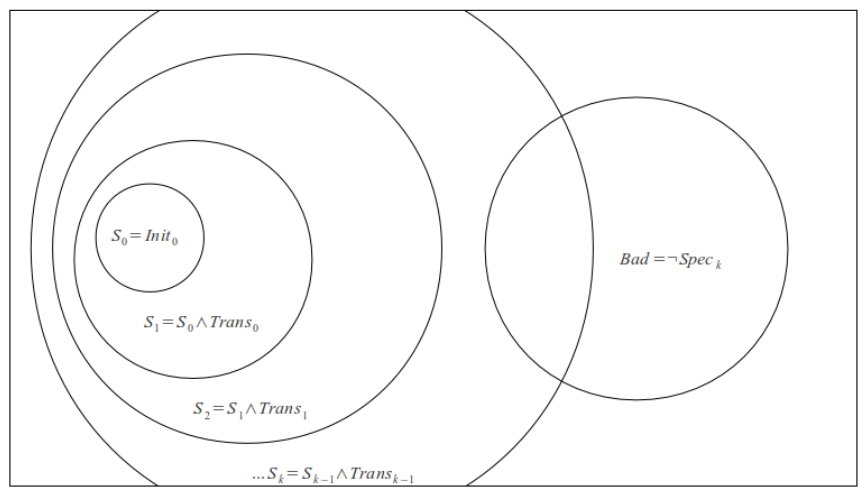
\includegraphics[scale=1]{bmc_example.png}
      \caption{Diagrama para funcionamento de BMC retirado de \cite[p. 16 ]{bachelor_thesis}.}
      \label{fig:bmc}
\end{figure}

Na figura ~\ref{fig:bmc}, está um diagrama que elucida a metodologia BMC.
Para um FOTS = $(Init, Trans)$, e uma propriedade $Spec$, a técnica de BMC
tenta verificar a atingibilidade de $\lnot Spec$ em até $k$ passos,
podendo apenas garantiar a segurança do sistema em traços finitos.

\section{\imc}
\label{state_of_art:imc}

O corpo de técnicas de IMC começou em \cite{interpolation_original}, com uma técnica para prova (ou refutação) de propriedades de FOTS através da utilização do interpolante de Craig, que se mostrou ser
favorável em comparação com as técnicas comuns à data da sua publicação, que se baseavam
também nas BDDs referidas acima.

No entanto, a restrição aqui é de apenas se considerarem FOTS finitos, que são os aplicáveis
à verificação de circuitos e ``\textit{hardware}'' industrial \textemdash para modelar
programas de software para o ramo da verificação formal, estes geralmente tomam a forma de
FOTS infinitos.\\

Em \cite{interpolation_state_of_art}, que foi uma das referências inicias dadas pelo
Professor Valença, construiu-se sobre \cite{interpolation_original} para permitir
FOTS infinitos, com o intuito de aplicar a técnica à verificação de ``\textit{software}''.
Fez-se novamente uma análise do desempenho que comprovou a viabilidade da técnica
numa suite de instâncias não-triviais de problemas-teste \footnote{\url{https://github.com/sosy-lab/benchexec}}.\\

Tem-se também o trabalho presente em \cite{interpolation_thesis}, que construindo
sobre \cite{interpolation_original} faz várias contribuições adicionais ao estabelecer
resultados teóricos sobre IMC, entre eles:
\begin{itemize}
    \item Todos os interpolantes gerados durante o IMC são aproximações, pelo que
    a sua precisão vai influenciar a velocidade da convergência do algoritmo até
    se chegar à indutividade da fórmula ou contra-exemplo.
    Este trabalho sistematiza formas de gerar interpolantes com propriedades
    e ``força'' (no sentido lógico, WPC/SPC) desejadas.
    \item À interpolação de fórmulas podem ser impostas propriedades específicas
    para garantir o funcionamento de uma dada técnica baseada em IMC. Esta obra
    estabelece relações entres as diversas propriedades, e uma hierarquia entre elas,
    que, relacionada com o ponto anterior, permitirá a construção de algoritmos
    de IMC ``genéricos'' com uma componente modular no algoritmo de interpolação
    utilizado, consoante o resultado que se pretende obter.
\end{itemize}

As inovações descritas nesta obra encontram-se em \cite{interpolation_thesis}, capítulo 1.3.

\begin{figure}[H]
      \centering
      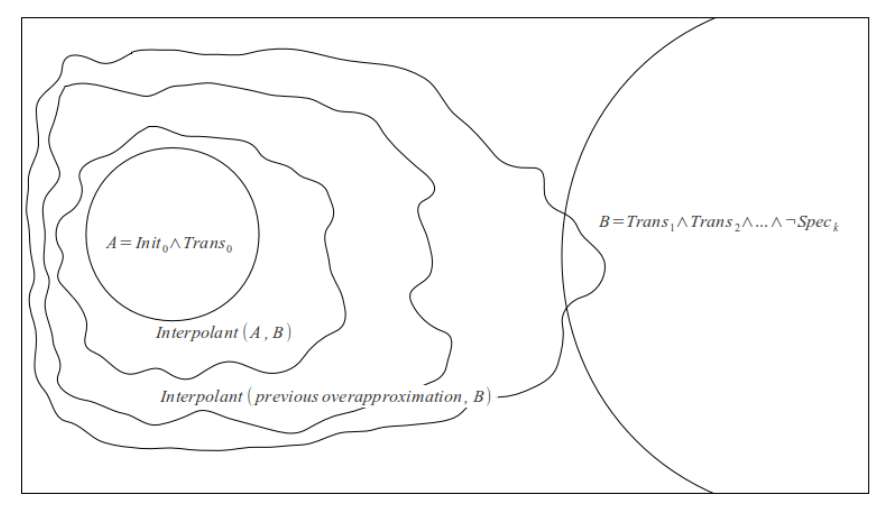
\includegraphics[scale=1]{imc_example.png}
      \caption{Diagrama para funcionamento de IMC retirado de \cite[p. 17] {bachelor_thesis}.}
      \label{fig:imc}
\end{figure}

Na figura ~\ref{fig:imc}, exemplifica-se a versão mais simples desta técnica.
Para um FOTS = $(Init, Trans)$, e uma propriedade $Spec$, a técnica de IMC
prova a validade de $Spec$ se for consistente com alguma ``overapproximation'' de
$Init \land Trans$ indutiva (obtidas através de interpolação).
Ao contrário do BMC, não se limita a traços infinitos, embora em  \cite{interpolation_original}
McMillan prova um limite superior às iterações necessárias para se atingir um
estado indutivo, ou a refutação.

\section{\pdr}
\label{state_of_art:pdr}

A técnica \pdr é introduzido em \cite{pdr_original}, com o ``\textit{caveat}'' de não
suportar, nesta descrição inicial, sistemas de transição de estados infinitos.
Baseia-se principalmente na noção de ``generalização indutiva'', descrita em
\cite{inductive_general}.

Consecutivo a \cite{pdr_original} vem \cite{pdr_efficient}, que apresenta melhorias
à implementação e desempenho do algoritmo PDR original, e discute a possibilidade de
melhoramentos adicionais futuros.\\

Para poder utilizar PDR em sistemas de estados infinitos \textemdash e daí poder trabalhar
com FOTS que representem programas, e fazer verificação formal \textemdash, é necessário
generalizar para FOTS de estados infinitos, o que foi feito em \cite{pdr_state_of_art}.
Isto requer uma combinação de interpolação, \kind e o PDR original.
Foi esta a referência dada aos autores para começar o estudo deste tópico.

\subsection*{CTIGAR e IC3}

A título complementar, mas sem ligação direta a este trabalho, nota-se que
em \cite{ic3} está uma introdução à primeira implementação de um ``\textit{model checker}''
baseado no PDR de \cite{pdr_original} pelo próprio autor.\\

Em \cite{ctigar} descreveu-se uma extensão do IC3 apta para sistemas de transição com estados
infinitos nomeada CTIGAR.

O IC3 foi ainda alvo de trabalho adicional em \cite{ic3_vienna} que, baseado em
\cite{ctigar}, desenvolveu outra extensão do IC3 original que também pode lidar com
sistemas de transição de estados infinitos.

\chapter{Análise do trabalho}
\label{chap:analysis}

Neste capítulo estará uma breve análise do trabalho feito, assim como algumas das
decisões tomadas na implementação de cada uma das técnicas de verificação,
assim como exemplos dessa implementação em PySMT quando não forem extensos demais.\\

Nota-se que todo o código aqui referenciado estará disponível no anexo em
~\ref{apndx:samples}, assim como no GitHub em ~\ref{apndx:github}.

\section{\kind e \bmc}
\label{analysis:kindbmc}

Para a \kind e \bmc, para além do trabalho feito nas aulas da UC de \lc
~\ref{state_of_art_lc_refs}, recorreu-se ao exemplo contido na documentação do 
PySMT\footnote{\url{https://pysmt.readthedocs.io/en/latest/tutorials.html#model-checking-an-infinite-state-system-bmc-k-induction-in-150-lines}}, que combina \kind e \bmc numa
só classe Python, que é construída a partir da representação em PySMT de um FOTS.
Este exemplo usa como referências \cite{bmc, kind_original}.\\

Apresenta-se de seguida um fragmento dessa classe com o método de verificação
de propriedades. A classe completa está em ~\ref{code:bmc_kind}.



\usemintedstyle{emacs}

\begin{code}
\begin{minted}{python}

class BMCInduction:
    def __init__(self, system):
        self.system = system

    ...

    def check_property(self, prop):
        """Interleaves BMC and K-Ind to verify the property."""
        print("Checking property %s..." % prop)
        from ply.cpp import xrange
        for b in xrange(100):
            f = self.get_bmc(prop, b)
            print("   [BMC]    Checking bound %d..." % (b + 1))
            if is_sat(f):
                print("--> Bug found at step %d" % (b + 1))
                return

            f = self.get_k_induction(prop, b)
            print("   [K-IND]  Checking bound %d..." % (b + 1))
            if is_unsat(f):
                print("--> The system is safe!")
                return

\end{minted}
\end{code}

Observe-se que esta implementação faz ``\textit{interleaving}'', ou ``entrelaçamento'',
das duas técnicas BMC e \kind, gerando traços sucessivamente maiores para o BMC, e só
no caso de sucesso com esta técnica se considera a utilização de $k$-indução, para
$k$ igual ao tamanho que se considera para os traços em cada momento, ou seja,
também crescente.

\section{\imc}
\label{analysis:imc}

Como foi descrito acima, considerou-se a implementação da interpolação presente em
\cite{interpolation_thesis}, pp. 38.

Em seguida está o pseudocódigo presente na citação acima:

\begin{figure}[H]
      \centering
      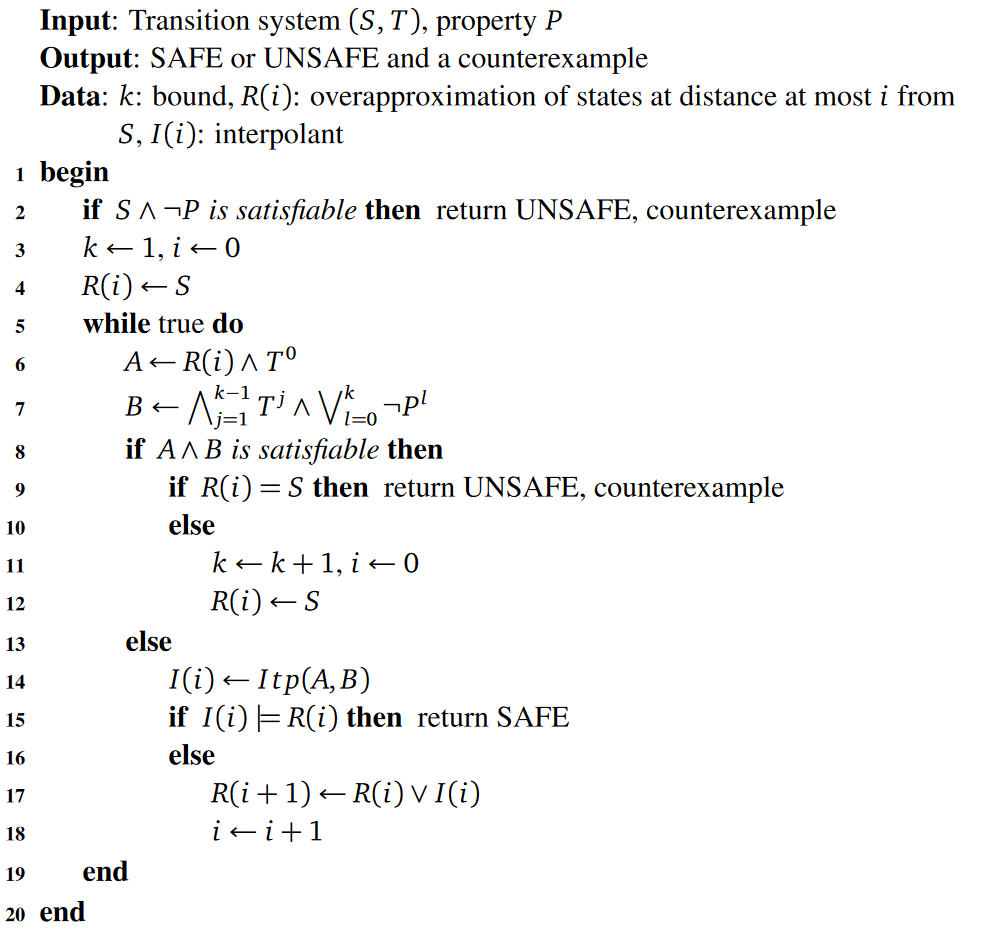
\includegraphics[scale=0.66]{imc-pseudocode.png}
      \caption{Pseudocódigo para IMC retirado de \cite{interpolation_thesis}}
      \label{fig:imcpseudo}
\end{figure}

Considere-se agora a implementação quase direta em Python, através do PySMT:

\begin{code}
\begin{minted}{python}
def IMC(S: Predicate,
        T: Predicate,
        P: Predicate,
        interpolator: Callable[[FNode, FNode], FNode] = binary_interpolant,
        print_info: bool = True):

    print("Checking if initial states violates safety property")
    if m := get_model(S[0] & ~P[0]):
        # halt return a counterexample
        if print_info:
            print(f"[step 0] Initial state violates property:")
            print(f"{INDENT}Counterexample:")
            print(textwrap.indent(f"{m}", INDENT))
        return Status.UNSAFE1

    k = 2

    i = 0
    R = S[0]

    while True:
        A = R & T[0]
        B = T[1:k - 1] & Or(~P[l] for l in range(k + 1))
        print(f"[{i=},{k=}] Checking BMC from R(i)")
        if m := get_model(A & B):
            if is_valid(EqualsOrIff(R, S[0])):
                print(f"[{i=},{k=}] Checking if R=S")
                print(m)
                return Status.UNSAFE2
            else:
                print(f"[{i=},{k=}] R != S")
                k += 1
                i = 0
                R = S[0]
        else:
            print(f"[{i=},{k=}] Calculating interpolant")
            I = interpolator(A, B)

            if is_valid(I.Implies(R)):
                if print_info:
                    print(f"[{i=},{k=}] Proved safety: all states have been covered, "
                          f"and the system is safe")
                return Status.SAFE
            else:
                print(f"[{i=},{k=}] I !=> R")
                R |= I
                i += 1
\end{minted}
\caption{Implementação em PySMT do algoritmo de IMC retirado de \cite{interpolation_thesis}}
\label{code:imc}
\end{code}

A versão com comentário encontra-se no anexo em~\ref{code:imc_commented}, ou no GitHub com
o resto do código fonte, também no anexo~\ref{apndx:github}.

\subsection{Problema da implementação em PySMT}
\label{imc:problem}

Nota-se que surgiu um problema com esta implementação que os autores lamentavelmente
não puderam resolver antes da data de submissão do projeto.
A função acima, relativamente ao FOTS em ~\ref{chap:case_study}, dava como válidas
propriedades obviamente falsas que o PDR em ~\ref{analysis:pdr} corretamente refutava.

Após várias tentativas de ``\textit{debugging}'', os autores suspeitam que se trate de uma,
ou mais, das seguintes situações:
\begin{itemize}
    \item O pseudocódigo de \cite{interpolation_thesis} apresenta alguma imprecisão \textemdash improvável.
    \item A função \href{https://pysmt.readthedocs.io/en/latest/api_ref.html#pysmt.shortcuts.is_valid}{\texttt{is_valid} tem um bug \textemdash provável devido à natureza ``\textit{open-source}'' do
    projeto, e à velocidade com a qual muda, sendo mais propenso a apresentar ``\textit{bugs}'' no software
    \item Um problema com a implementação acima~\ref{code:imc}, quer na transliteração do
    pseudocódigo para PySMT, quer nalgum detalhe de implementação \textemdash esta parece ser
    a mais provável, mas não se pôde confirmar a tempo da submissão.
\end{itemize}

\subsection{Interpolante de Craig, escolha de lógica SMT}
\label{imc_craig}

Para implementar este algoritmo, foi necessário utilizar o teorema de interpolação de
Craig\footnote{\url{https://en.wikipedia.org/wiki/Craig_interpolation}}, que já estava
\href{https://en.wikipedia.org/wiki/Craig_interpolation}{implementado no PySMT}.\\

É preciso notar que a implementação do PySMT não suporta todas as lógicas \smtlib.
Por exemplo, no ``caso de estudo'' apresentado em ~\ref{chap:case_study}, a lógica
$\textrm{QF\_BV}$ \footnote{\url{https://smtlib.cs.uiowa.edu/logics-all.shtml#QF_BV}}
é suficiente para considerar o problema.\\

No entanto, se não for \textbf{explicitamente} selecionada, o PySMT escolherá
a lógica mais geral que conseguir, que no caso era \begin{math}\textrm{QF\_AUFBVLIRA}\end{math}\footnote{\url{https://smtlib.cs.uiowa.edu/logics-all.shtml#QF_AUFLIA}}, que
não tem, à data da submissão do projeto, uma implementação de um algoritmo para
cálculo do interpolante de Craig entre duas fórmulas arbitrárias.

Isto significa que o utilizador da ferramenta tem a responsabilidade de escolher
manualmente a lógica apropriada para garantir o funcionamento desta implementação
de IMC.

\subsection{Interpolante utilizando noção de WPC e SPC, e linguagem de fluxos}
\label{imc_wpc_spc}

Como se referiu em ~\ref{chap:intro}, uma das propostas para a técnica do IMC
foi fazer a conversão de FOTS para programas num fragmento da \href{https://paper.dropbox.com/doc/Capitulo-5-Verificacao-Formal-de-Software-e95D7fVpc0dArh4pnVl1l#:uid=847823822173927851567448&h2=Denota%C3%A7%C3%A3o-WPC-e-sua-linguagem-}{linguagem de fluxos} estudada em \lc, e utilizar as metodologias de \wpc (WPC) e \spc (spc)
para obter interpolantes em vez do interpolante de Craig.

Elabora-se esta ideia de seguida.

\subsubsection{Relação entre linguagem de fluxos e FOTS}

Considere-se o seguinte programa simples retirado do material de LC\footnote{\url{https://paper.dropbox.com/doc/Capitulo-3-Satisfiability-Modulo-Theories-2-Parte-zorZj2G3ceOIi92zrE0n1}}:

\begin{code}
\begin{minted}{python}
assert (z >= 0)
0: while z > 0:
1:    z = z - 1
2: stop
\end{minted}
\caption{Exemplo de programa simples em Python}
\label{code:simple_prog}
\end{code}

Aplicando a metodologia estudada na UC de LC (que se explica no link anterior), isto dá
origem ao FOTS

\begin{figure}[H]
      \centering
      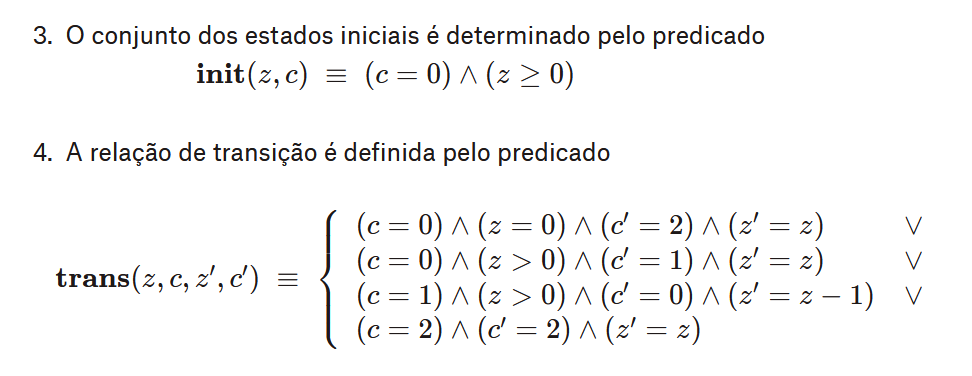
\includegraphics[scale=0.85]{simple_prog.png}
      \caption{Programa de \ref{code:simple_prog} convertido para FOTS}
      \label{fig:simple_fots}
\end{figure}

Pode-se também considerar aumentar o FOTS com um estado de erro, como exemplificado
em \cite{interpolation_state_of_art}. Para o exemplo acima, seria:

$$
\textbf{err}(z, c) \ \equiv \ (c = 2) \land (z > 0)
$$

Considere-se agora a tradução do FOTS acima para a linguagem de programas anotados.

\begin{code}
\begin{minted}{python}
{
assume c = 0 and z = 0;
c = 2;
} ||
{
assume c = 0 and z > 0;
c = 1;
} ||
{
assume c = 1 and z > 0;
c' = 0;
z = z - 1;
} ||
{
assume c = 2;
skip;
}
\end{minted}
\caption{Tradução de FOTS para LPA}
\label{code:fots_to_lpa}
\end{code}

Observe-se uma das razões para se considerar o IMC neste formato - no caso de uma
transição não modificar uma variável do FOTS, ela não precisará ser incluída no
programa LPA, levando a programas mais pequenos, que por si levarão depois a fluxos
menores, e logo fórmulas mais simples que potenciam melhor desempenho.

A representação normal de um FOTS obriga à inclusão de todas as variáveis em todas as
transições.\\

Note-se que esta tradução nem sempre é possível - no caso de o FOTS em causa representar
um \href{https://paper.dropbox.com/doc/Capitulo-4-Sistemas-Hibridos-ycW40nf36f1eZW4f4k5e8}{sistema ciber-físico},
algumas das suas transições poderão não ser representáveis no fragmento da LPA que apenas
contém atribuições e \texttt{assume}s.
Isto acontece porque no caso das transições ``\textit{timed}'', a discretização das
equações diferenciais que regem a transição poderá não ser representável no fragmento
da LPA que se escolheu.\\

Seja $Prog$ o fluxo gerado do programa acima, e considere-se agora uma esquematização do IMC com LPA.

\begin{figure}[H]
\centering
\begin{tikzpicture}[shorten >=1pt,node distance=3cm,on grid, auto, initial text = ]

  \node[state] (Sk) {$\phi_?$};
  \node[state] (In) [left=of Sk]{$\text{SP}_T(I)$};
  \node[state] (En) [right=of Sk]{$\text{WP}_T(E)$};
  \node[state, initial left] (I1) [left=of In]{I};
  \node[state, initial right] (E1) [right=of En]{E};
  
  \path[->]
    (I1) edge node {SPC} (In)
    (E1) edge node {WPC} (En);

  \path
    (En) -- node[auto=false]{\ldots} (Sk);

  \path
    (In) -- node[auto=false]{\ldots} (Sk);

\end{tikzpicture}
\caption{Interpolante em programas LPA com WPC/SPC}
\label{fig:lpa_wpc_spc}
\end{figure}

A ideia é partir dos dois estados, $I$ e $E$, e ir sucessivamente aplicando as
regras WPC/SPC descritas em \footnote{\url{https://paper.dropbox.com/doc/Capitulo-5-Verificacao-Formal-de-Software-e95D7fVpc0dArh4pnVl1l#:uid=847823822173927851567448&h2=Denota\%C3\%A7\%C3\%A3o-WPC-e-sua-linguagem-}},
\footnote{\url{https://paper.dropbox.com/doc/Capitulo-5-Verificacao-Formal-de-Software-e95D7fVpc0dArh4pnVl1l#:uid=999909737185703645851102&h2=Denota\%C3\%A7\%C3\%A3o-SPC-(\%E2\%80\%9Cstrongest-post}}
para ir gerando novos predicados, e ver se eles alguma vez se intersectam para provar
a validade da propriedade $P$ que se quer provar:

\begin{itemize}
    \item Se $\phi_?$ existir, ou seja, se houver algum estado alcançável simultaneamente
    a partir de $I$ (através de SPC) e de $E$ (através de WPC), então o sistema é inseguro
    \item Se $\phi_?$ não existir, ou seja, se se chegar a estados $I_k, E_k$ que sejam
    indutivos e não sejam equivalentes, e tais que $I_k$ seja consistente com $P$, então
    o sistema é seguro, e a propriedade é válida.
\end{itemize} 

Para entender este conceito, recorreu-se a \cite{interpolant_spc_wpc}.

Esta ideia \textbf{não} foi implementada na ferramenta, mesmo após uma contribuição inicial do
Professor Valença. No entanto, deixou-se o código não funcional no GitHub para
referência futura; está indicado em ~\ref{apndx:github}.

\section{\pdr}
\label{analysis:pdr}

Na documentação da ferramenta PySMT, para além de implementações das técnicas \kind e
\bmc --- ver ~\ref{analysis:kindbmc} ---, existe também uma implementação básica de PDR
(vinda de \cite{pdr_original}) que serviu aos autores para entender o funcionamento do método.\\

No entanto, essa implementação apenas suporta FOTS com um número de estados \textbf{finito}.
Assim sendo, para suportar FOTS infinitos, é necessário outro algoritmo.
Foi referido na introdução~\ref{intro:pdr} que se consideraram duas formas de implementar
a técnica de PDR para FOTS infinitos:

\begin{itemize}
    \item Uma em \cite{ctigar} (capítulo 3)
    \item A outra em \cite{pdr_state_of_art}, que foi a opção escolhida no final.
\end{itemize}

Em CTIGAR existem as noções de ``\textit{counterexamples to induction (CTIs)}'',
de ``\textit{abstraction}'' e ``\textit{consecution}'' --- ver ~\cite{ctigar}
(capítulos 2, 3).

Devido a dificuldades na implementação da noção de ``\textit{consecution}'', a partir da
implementação em Java do CTIGAR, optou-se pela segunda via do PDR.
Como no caso da metodologia SPC+WPC para o IMC~\ref{imc_wpc_spc}, manteve-se o código
resultante desta tentativa no GitHub do projeto ~\ref{apndx:github}.\\

Em seguida está o pseudocódigo presente em \cite{pdr_state_of_art}, que foi o ponto
de partida para a implementação em PySMT:

\begin{figure}[H]
      \centering
      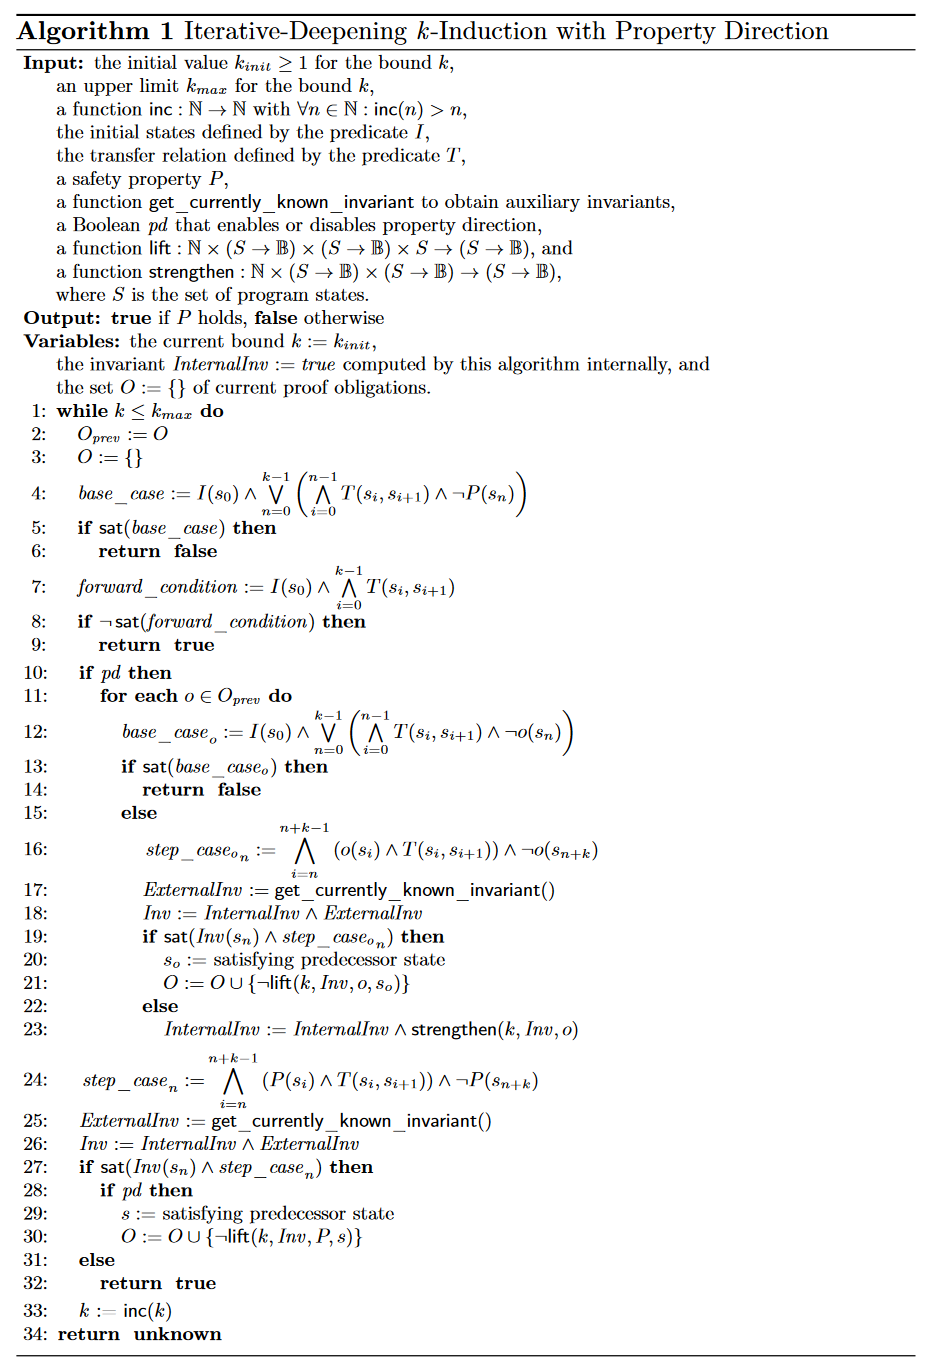
\includegraphics[scale=0.75]{pdr-pseudocode.png}
      \caption{Pseudocódigo para PDR retirado de \cite{pdr_state_of_art}}
      \label{fig:pdrpseudo}
\end{figure}

Considere-se agora a implementação quase direta do pseucódigo acima em PySMT:

\begin{code}
\begin{minted}{python}
def PDR(I: Predicate,
        T: Predicate,
        P: Predicate,
        get_currently_known_invariant=lambda: TRUE(),
        strengthen=lambda k, Inv, o: Inv,
        lift=_lift,
        k_init: int = 1,
        k_max: int = float('inf'),
        pd: bool = True,
        inc: Callable[[int], int] = lambda n: n + 1,
        print_info=True
        ) -> bool | Status:
    k: int = k_init

    InternalInv: FNode = TRUE()

    O: Set[Predicate] = set()

    while k <= k_max:
        O_prev: Set[Predicate] = O
        O = set()

        # begin: base-case check (BMC)
        base_case = get_base_case(k, I, T, P)
        if m := get_model(base_case):
            if print_info:
                print(f"[{k=}] base-case check failed")
                print(f"{INDENT}Counterexample:")
                print(textwrap.indent(f"{str_model(m)}", INDENT))
            return False
        # end ############################################################################

        # begin: forward-condition check (as described in Sec. 2)
        forward_condition = I[0] & T[:k - 1]
        if is_unsat(forward_condition):
            print(f"[{k=}] Proved correctness: successful forward condition check")
            pprint(forward_condition.serialize())
            return True
        # end ############################################################################

        # begin: attempt to prove each proof obligation using k-induction
        if pd:
            for o in O_prev:
                # begin: check the base case for a proof obligation o
                base_case_o = get_base_case(k, I, T, o)
                if is_sat(base_case_o):
                    print(f"[{k=}] Found violation for proof obligation {o}")
                    return False
                # end ####################################################################

                else:
                    # no violation was found

                    # begin: check the inductive-step case to prove o
                    step_case_o_n = get_step_case(k, T, o)
                    ExternalInv = get_currently_known_invariant()
                    Inv = Predicate(InternalInv & ExternalInv)
                    if m := get_model(Inv[0] & step_case_o_n):
                        s_o = Predicate(get_assignment_as_formula_from_model(m))
                        predicate_describing_set_of_CTI_states = lift(k, Inv, P, s_o, T)
                        if predicate_describing_set_of_CTI_states:
                            O = O.union(Not(predicate_describing_set_of_CTI_states))
                    else:
                        InternalInv &= strengthen(k, Inv, o)
                    # end ################################################################
        # end: attempt to prove each proof obligation using k-induction

        # begin: check the inductive-step case for the safety property P
        step_case_n = get_step_case(k, T, P)
        ExternalInv = get_currently_known_invariant()
        Inv = Predicate(InternalInv & ExternalInv)
        if m := get_model(Inv[0] & step_case_n):
            if pd:
                s = get_assignment_as_formula_from_model(m)
                # Try to lift this state to a more abstract state that still satisfies
                # the property that all of its successors violate the safety property.
                if abstract_state := lift(k, Inv, P, Predicate(s), T):
                    O = O.union(Not(abstract_state))
        else:
            print(f"[{k=}] Proved correctness: safety property is inductive")
            return True
        # end ############################################################################

        k = inc(k)
    print("Property's status is unknown: exceeded maximum number of iterations")
    return Status.UNKNOWN\end{minted}
\caption{Implementação em PySMT do algoritmo de PDR retirado de \cite{pdr_state_of_art}}
\label{code:pdr}
\end{code}

A versão original com comentários encontra-se no anexo em ~\ref{code:pdr_commented}.
Como no caso do IMC, o PySMT facilita a prototipagem de funções a partir de pseudocódigo
de forma quase imediata.\\

\section*{Notes sobre a implementação do PDR}
\label{pdr:notes}

Veja-se que no pseudocódigo em ~\ref{fig:pdrpseudo}, a função para o PDR recebe
transformadores de predicados como argumentos: $lift, strengthen$.
Devido a limitações de tempo, não se pôde considerar os tranformadores descritos
em \cite{pdr_state_of_art}, pelo que usa-se a identidade para $strengthen$ por omissão.

\chapter{Caso de Estudo}\label{chap:case_study}

Para testar a ferramenta desenvolvida, escolheu-se um exemplo de um programa sem
grande complexidade, mas não trivial, de um \fots visto num dos trabalhos práticos da UC de 
\href{https://paper.dropbox.com/doc/LC-2021-2022-Trabalhos-Praticos-NZEwyS6N5YQQTw1XsYimE#:uid=036036509450795602269559&h2=Trabalho-4}{\lc}.

\begin{figure}[H]
      \centering
      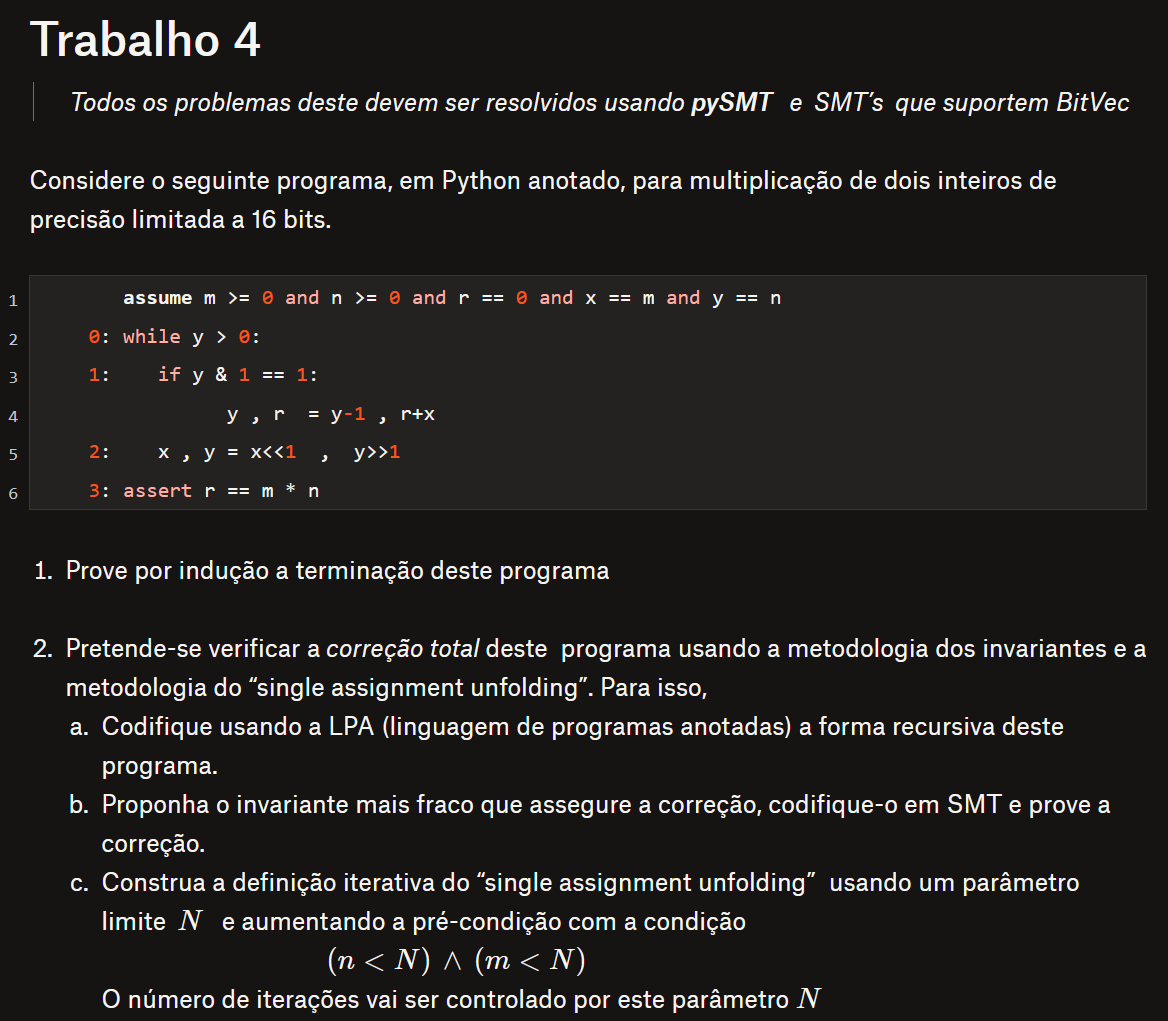
\includegraphics[scale=0.68]{lc-trab4.png}
      \caption{FOTS de trabalho 4 de \lc, ano letivo 2021/2022}
      \label{fig:trab4}
\end{figure}

Na documentação referenciada no anexo ~\ref{apndx:example} apresenta-se um FOTS para o programa em
~\ref{fig:trab4}, e mostra-se um exemplo de utilização da ferramenta para provar algumas propriedades
sobre ele.

\chapter{Conclusão} \label{chap:concl}

Conclui-se desta forma a apresentação do trabalho desenvolvido pelos autores
para a UC \proj no ano letivo 2021/2022.

\section{Comentários}

Os autores concluem, após terminar o projeto, que as capacidades oferecidas
pelo PySMT são boas, e que é uma ferramenta capaz de implementar conceitos
complexos sem grande dificuldade.\\

No entanto, a documentação oferecida pelo projeto é esparsa, e quando existe
é muitas vezes insuficiente. Fruto de ser um projeto ``\textit{open-source}'',
é alvo de constantes mudanças, o que tornam a biblioteca inapropriada para
projetos sérios que vão além de prototipagem. Veja-se por exemplo o erro
``silencioso'' que se obtinha em ~\ref{imc_craig} fruto de permitirà biblioteca
deduzir a escolha da lógica SMT

Referenciada em várias das obras consultadas para este projeto (\cite{ctigar, kind_state_of_art, interpolation_state_of_art},
a ferramenta \cpa seria uma alternativa a considerar para trabalhos futuros
deste género.

\section{Trabalho Futuro}

Por ser um projeto académico a nível de licenciatura, é improvável que veja
qualquer uso futuro adicional.

No entanto, há várias possibilidades para o melhorar:
\begin{itemize}
    \item Mais importante que todas outras, referenciada em ~\ref{imc:problem} \textemdash
    corrigir o problema com a implementação do IMC em PySMT, que leva o algoritmo
    a dar, por vezes, resultados incorretos.
    \item Implementar a ideia de IMC através de WPC+SPC descrita em ~\ref{imc_wpc_spc}
    \begin{itemize}
        \item Esta própria ideia poderia ser melhorada ao implementar um algoritmo
        dinâmico de escolha de metodologia de prova IMC para usar a técnica adequada
        para um dado FOTS
        \item Testes comparativos ao desempenho das duas técnicas também seriam
        esclarecedores
    \end{itemize}
    \item Como mencionado em ~\ref{analysis:pdr}, teria sido positivo terminar a
    implementação do PDR semelhante àquela que o CTIGAR usa, descrita em \cite{ctigar}, assim como comparar o desempenho das duas técnicas
    \item Teria também sido relevante estudar o efeito de transformadores
    descritos em ~\ref{pdr:notes} de predicados adicionais no comportamento
    do PDR.
\end{itemize}

\appendix % apendice
\chapter{Excertos de Código Utilizado no Projeto} \label{apndx:samples}

\section{\kind combinada com \bmc}

\begin{code}
\begin{minted}{python}

class BMCInduction:
    def __init__(self, system):
        self.system = system

    def get_simple_path(self, k):
        """Simple path constraint for k-induction:
        each time encodes a different state
        """
        res = []
        for i in range(k + 1):
            subs_i = self.system.get_subs(i)
            for j in range(i + 1, k + 1):
                state = []
                subs_j = self.system.get_subs(j)
                for v in self.system.variables:
                    v_i = v.substitute(subs_i)
                    v_j = v.substitute(subs_j)
                    state.append(Not(EqualsOrIff(v_i, v_j)))
                res.append(Or(state))
        return And(res)

    def get_k_hypothesis(self, prop, k):
        """Hypothesis for k-induction: each state up to k-1 fulfills the property"""
        res = []
        for i in range(k):
            subs_i = self.system.get_subs(i)
            res.append(prop.substitute(subs_i))
        return And(res)

    def get_bmc(self, prop, k):
        """Returns the BMC encoding at step k"""
        init_0 = self.system.init.substitute(self.system.get_subs(0))
        prop_k = prop.substitute(self.system.get_subs(k))
        return And(self.system.get_unrolling(k), init_0, Not(prop_k))

    def get_k_induction(self, prop, k):
        """Returns the K-Induction encoding at step K"""
        subs_k = self.system.get_subs(k)
        prop_k = prop.substitute(subs_k)
        return And(self.system.get_unrolling(k),
                   self.get_k_hypothesis(prop, k),
                   self.get_simple_path(k),
                   Not(prop_k))

    def check_property(self, prop):
        """Interleaves BMC and K-Ind to verify the property."""
        print("Checking property %s..." % prop)
        from ply.cpp import xrange
        for b in xrange(100):
            f = self.get_bmc(prop, b)
            print("   [BMC]    Checking bound %d..." % (b + 1))
            if is_sat(f):
                print("--> Bug found at step %d" % (b + 1))
                return

            f = self.get_k_induction(prop, b)
            print("   [K-IND]  Checking bound %d..." % (b + 1))
            if is_unsat(f):
                print("--> The system is safe!")
                return
\end{minted}
\caption{Implementação do algoritmo de BMC + \kind retirada de \href{https://pysmt.readthedocs.io/en/latest/tutorials.html##model-checking-an-infinite-state-system-bmc-k-induction-in-150-lines}{documentação de PySMT}}
\label{code:bmc_kind}
\end{code}

\section{\imc}

\begin{code}
\begin{minted}{python}
def IMC(S: Predicate,
        T: Predicate,
        P: Predicate,
        interpolator: Callable[[FNode, FNode], FNode] = binary_interpolant,
        print_info: bool = True):
    """
    Interpolating Model Checking

    As specified at S. Fulvio Rollini, “Craig Interpolation and Proof Manipulation:
    Theory and Applications to Model Checking,” Università della Svizzera Italiana. p.
    38. available at https://verify.inf.usi.ch/sites/default/files/RolliniPhDThesis.pdf

    A property to be verified is encoded as a formula :math:`P` , so that the system is
    safe if the error states where :math:`¬P` holds are not reachable from :math:`S`.

    Verifying that the system satisfies :math:`P` reduces to prove
    that :math:`P` is an inductive invariant property:

    .. math:: S ⊨ P\\qquad P ∧ T ⊨ P'

    If (i) the initial states satisfy :math:`P` and, (ii) assuming :math:`P` holds,
    it also holds after applying the transition relation, then :math:`P` holds in all
    reachable states. When the inductiveness of :math:`P` cannot be directly proved,
    it might be possible to show that another formula :math:`\\hat P`, stronger than
    :math:`P ( \\hat P ⊨ P )`, is an inductive invariant, from which :math:`P` would
    follow as a consequence; this algorithm, which combines interpolation and bounded
    model checking (BMC), is based on iteratively building such a :math:`\\hat P`.
    """

    # first makes sure P is not violated by S
    print("Checking if initial states violates safety property")
    if m := get_model(S[0] & ~P[0]):
        # halt return a counterexample
        if print_info:
            print(f"[step 0] Initial state violates property:")
            print(f"{INDENT}Counterexample:")
            print(textwrap.indent(f"{m}", INDENT))
        return Status.UNSAFE1

    # bound
    k = 2

    # overapproximation of states at distance at most i from S
    i = 0
    R = S[0]

    # for a bound k and a current overapproximation R(i) of the states at distance at
    # most i from S, the algorithm checks if P is violated by the states reachable
    # from R(i) in at most k steps.
    while True:
        A = R & T[0]
        B = T[1:k - 1] & Or(~P[l] for l in range(k + 1))
        print(f"[{i=},{k=}] Checking BMC from R(i)")
        if m := get_model(A & B):
            # the error might be real or spurious, caused by an insufficient value of k
            if is_valid(EqualsOrIff(R, S[0])):
                print(f"[{i=},{k=}] Checking if R=S")
                # error is real so the system is unsafe
                print(m)
                return Status.UNSAFE2
            else:
                # error is spurious so k is increased to allow finer
                # overapproximations, and the algorithm restarts from S.
                print(f"[{i=},{k=}] R != S")
                k += 1
                i = 0
                R = S[0]
        # R(i) ⋀_{j=0}^{k−1} T^j ⋁_{l=0}^k ¬P^l is unsat
        else:
            # an interpolant I(i) is computed, which represents an approximation of the
            # image of R(i) (i.e., of the states reachable from R(i) in one step).
            print(f"[{i=},{k=}] Calculating interpolant")
            I = interpolator(A, B)

            # a fixpoint check is carried out: if I(i) |= R(i), it means that all
            # states have been covered, and the system is safe; otherwise, R(i + 1) is
            # set to R(i) ∨ I(i) and the procedure continues.
            if is_valid(I.Implies(R)):
                # the current R(i) corresponds to an inductive invariant P̂ stronger
                # than P: on one side, S |= R(i), moreover R(i) ∧ T |= I'(i) and I(i)
                # |= R(i) imply R(i) ∧ T |= R'(i); on the other side, the fact that at
                # each iteration 0 ≤ h ≤ i, R(h) ∧ ⋀_{j=0}^{k−1} T |= ⋀_{l=0}^k P^l,
                # together with R(i) being an inductive invariant, yield R(i) |= P.
                if print_info:
                    # print(f"R({i}) = ", R.simplify().serialize())
                    print(f"[{i=},{k=}] Proved safety: all states have been covered, "
                          f"and the system is safe")
                return Status.SAFE
            else:
                print(f"[{i=},{k=}] I !=> R")
                R |= I
                i += 1
\end{minted}
\caption{Implementação comentada do algoritmo de IMC -\cite{interpolation_thesis}}
\label{code:imc_commented}
\end{code}

\section{\pdr}

\begin{code}
\begin{minted}{python}
def PDR(I: Predicate,
        T: Predicate,
        P: Predicate,
        get_currently_known_invariant=lambda: TRUE(),
        strengthen=lambda k, Inv, o: Inv,
        lift=_lift,
        k_init: int = 1,
        k_max: int = float('inf'),
        pd: bool = True,
        inc: Callable[[int], int] = lambda n: n + 1,
        print_info=True
        ) -> bool | Status:
    """
    Iterative-Deepening k-Induction with Property Direction.

    As specified at D. Beyer and M. Dangl, “Software Verification with PDR:
    Implementation and Empirical Evaluation of the State of the Art” arXiv\:1908.06271
    [cs], Feb. 2020, Accessed: Mar. 05, 2022. [Online]. Available
    https://arxiv.org/abs/1908.06271.

    :param print_info: Whether info about the steps should be printed.
    :param k_init: the initial value :math:`≥1` for the bound `k`
    :param k_max: an upper limit for the bound `k`
    :param inc: a function :math:`ℕ → ℕ` such that :math:`∀n ∈ ℕ: \\inc(n) > n`
    :param TS: Contains predicates defining the initial states and the transfer relation
    :param P: The safety property
    :param get_currently_known_invariant: used to obtain the strongest invariant currently
        available via a concurrently running (external) auxiliary-invariant generator
    :param pd: boolean flag pd (reminding of “property-directed”) is used to control
        whether failed induction checks are used to guide the algorithm towards a
        sufficient strengthening of the safety property P to prove correctness; if pd is
        set to false, the algorithm behaves exactly like standard k-induction.
    :param lift: Given a failed attempt to prove some candidate invariant :math:`Q` by
        induction, the function lift is used to obtain from a concrete
        counterexample-to-induction (CTI) state a set of CTI states described by a state
        predicate C. An implementation of the function :math:`k ∈ ℕ, \\Inv ∈ ℕ × (S →
        ��) × (S → ��) × S → (S → ��)` and :math:`C = \\lift(k, \\Inv , Q, s)`, lift needs to
        satisfy the condition that for a CTI :math:`s ∈ S` where :math:`S` is the set of
        program states, the following holds:

        .. math:: C(s) ∧ \\left( ∀s_n ∈ S: C(s_n) ⇒\
            \\Inv(s_n) ∧
            \\displaystyle\\bigwedge_{i=n}^{n+k−1} (Q(s_i) ∧ T(s_i ,s_{i+1})) ⇒ ¬Q(s_{n+k}) \\right)

        which means that the CTI s must be an element of the set of states described by
        the resulting predicate C and that all states in this set must be CTIs, i.e.,
        they need to be k-predecessors of :math:`¬Q`-states, or in other words,
        each state in the set of states described by the predicate :math:`C` must reach
        some :math:`¬Q`-state via :math:`k` unrollings of the transition relation
        :math:`T`.
    :param strengthen: The function strengthen: :math:`ℕ × (S → ��) × (S → ��) → (S →
        ��)` is used to obtain for a k-inductive invariant a stronger k-inductive
        invariant, i.e., its result needs to imply the input invariant, and, just like the
        input invariant, it must not be violated within k loop iterations and must be
        k-inductive.
    :return: `True` if `P` holds, `Status.UNKNOWN` if `k > k_max` , `False` otherwise.
    """

    # current bound
    k: int = k_init

    # the invariant computed by this algorithm internally
    InternalInv: FNode = TRUE()

    # the set of current proof obligations.
    O: Set[Predicate] = set()

    while k <= k_max:
        O_prev: Set[Predicate] = O
        O = set()

        # begin: base-case check (BMC)
        #
        # Base Case. The base case of k-induction consists of running BMC with the
        # current bound k. This means that starting from all initial program states, all
        # states of the program reachable within at most k−1 unwindings of the transition
        # relation are explored. If a ¬P-state is found, the algorithm terminates.
        base_case = get_base_case(k, I, T, P)
        if m := get_model(base_case):
            if print_info:
                print(f"[{k=}] base-case check failed")
                print(f"{INDENT}Counterexample:")
                print(textwrap.indent(f"{str_model(m)}", INDENT))
                # print(textwrap.indent(f"{m}", INDENT))
            return False
        # end ############################################################################

        # begin: forward-condition check (as described in Sec. 2)
        #
        # Forward Condition. If no ¬P-state is found by the BMC in the base case, the
        # algorithm continues by performing the forward-condition check, which attempts
        # to prove that BMC fully explored the state space of the program by checking
        # that no state with distance k′ > k−1 to the initial state is reachable. If this
        # check is successful, the algorithm terminates.
        forward_condition = I[0] & T[:k - 1]
        if is_unsat(forward_condition):
            print(f"[{k=}] Proved correctness: successful forward condition check")
            pprint(forward_condition.serialize())
            return True
        # end ############################################################################

        # begin: attempt to prove each proof obligation using k-induction
        if pd:
            for o in O_prev:
                # begin: check the base case for a proof obligation o
                base_case_o = get_base_case(k, I, T, o)
                if is_sat(base_case_o):
                    # If any violations of the proof obligation o are found, this means
                    # that a predecessor state of a ¬P-state, and thus, transitively,
                    # a ¬P -state, is reachable, so we return false.
                    print(f"[{k=}] Found violation for proof obligation {o}")
                    return False
                # end ####################################################################

                else:
                    # no violation was found

                    # begin: check the inductive-step case to prove o
                    #
                    # Inductive-Step Case. The forward-condition check, however,
                    # can only prove safety for programs with finite (and, in practice
                    # short) loops. To prove safety beyond the bound k, the algorithm
                    # applies induction: The inductive-step case attempts to prove tha
                    # after every sequence of k unrollings of the transition relation
                    # that did not reach a ¬P-state, there can also be no subsequent
                    # transition into a ¬P-state by unwinding the transition relation
                    # once more. In the realm of model checking of software, however,
                    # the safety property P is often not directly k-inductive for any
                    # value of k, thus causing the inductive-step-case check to fail.
                    # It is therefore state-of-the-art practice to add auxiliary
                    # invariants to this check to further strengthen the induction
                    # hypothesis and make it more likely to succeed. Thus,
                    # the inductive-step case proves a program safe if the following
                    # condition is unsatisfiable:
                    #
                    #   Inv(s_n) ⋀_{i=n}^{n+k-1}(P(s_i) ∧ T(s_i,s_{i+1})) ∧ ¬P(s_{n+k})
                    #
                    # where Inv is an auxiliary invariant, and sₙ,…,sₙ₊ₖ is any
                    # sequence of states. If this check fails, the induction attempt is
                    # inconclusive, and the program is neither proved safe nor unsafe
                    # yet with the current value of k and the given auxiliary
                    # invariant. In this case, the algorithm increases the value of k
                    # and starts over.
                    step_case_o_n = get_step_case(k, T, o)
                    ExternalInv = get_currently_known_invariant()
                    Inv = Predicate(InternalInv & ExternalInv)
                    if m := get_model(Inv[0] & step_case_o_n):
                        s_o = Predicate(get_assignment_as_formula_from_model(m))
                        predicate_describing_set_of_CTI_states = lift(k, Inv, P, s_o, T)
                        if predicate_describing_set_of_CTI_states:
                            O = O.union(Not(predicate_describing_set_of_CTI_states))
                    else:
                        # If the step-case check for o is successful,
                        # we no longer track o in the set O of unproven proof obligations.

                        # We could now directly use the proof obligation as an
                        # invariant, but instead, we first try to strengthen it into a
                        # stronger invariant that removes even more unreachable states
                        # from future consideration before conjoining it to our
                        # internally computed auxiliary invariant. In our
                        # implementation, we implement strengthen by attempting to drop
                        # components from a (disjunctive) invariant and checking if the
                        # remaining clause is still inductive.
                        InternalInv &= strengthen(k, Inv, o)
                    # end ################################################################
        # end: attempt to prove each proof obligation using k-induction

        # begin: check the inductive-step case for the safety property P
        #
        # This check is mostly analogous to the inductive-step case check for the proof
        # obligations described above, except that if the check is successful,
        # we immediately return true.

        # Assume for any iteration n (k iterations from n to n + k − 1 = n) that the
        # safety property holds, and from this assumption attempt to conclude that the
        # safety property will also hold in the next iteration n + 1 (n + k).
        step_case_n = get_step_case(k, T, P)
        ExternalInv = get_currently_known_invariant()
        Inv = Predicate(InternalInv & ExternalInv)
        if m := get_model(Inv[0] & step_case_n):
            if pd:
                s = get_assignment_as_formula_from_model(m)
                # Try to lift this state to a more abstract state that still satisfies
                # the property that all of its successors violate the safety property.
                if abstract_state := lift(k, Inv, P, Predicate(s), T):
                    # Negate this abstract state to obtain the proof obligation.
                    # This means that we have learned that we should prove the
                    # invariant ¬o, such that in future induction checks, we can remove
                    # all states that satisfy `o` from the set of predecessor states
                    # that need to be considered.
                    O = O.union(Not(abstract_state))
        else:
            print(f"[{k=}] Proved correctness: safety property is inductive")
            return True
        # end ############################################################################

        k = inc(k)
    print("Property's status is unknown: exceeded maximum number of iterations")
    return Status.UNKNOWN
\end{minted}
\caption{Implementação comentada do algoritmo de PDR -\cite{pdr_state_of_art}}
\label{code:pdr_commented}
\end{code}

\chapter{Repositório \textit{GitHub} com código fonte e documentação} \label{apndx:github}

\section*{``\textit{Source code}''}

O código fonte da ferramenta desenvolvida é accessível através do link: \url{https://github.com/Alef-Keuffer/FOTS-Prover}.

Está sediado numa página de GitHub de um dos autores.

\section*{Implementações incompletas}

Como referido em  \label{analysis:pdr, imc_wpc_spc}, as implementações incompletas do IMC
através de WPC/SPC, e do PDR baseasdo em CTIGAR de \cite{ctigar} estão em: \url{https://github.com/Alef-Keuffer/FOTS-Prover/tree/main/src/unfinished}.

\section*{Documentação da ferramenta}

A documentação da ferramenta encontra-se disponível \href{https://alef-keuffer.github.io/FOTS-Prover.docs/index.html}{aqui}.

\subsection*{Documentação de exemplo}
\label{apndx:example}

A documentação do exemplo em ~\ref{chap:case_study} está 
\href{https://alef-keuffer.github.io/FOTS-Prover.docs/examples.trab4.html}{aqui}.

\newpage

%-- Fim do documento -- inserção das referencias bibliográficas

%\bibliographystyle{plain} % [1] Numérico pela ordem de citação ou ordem alfabetica
\bibliographystyle{IEEEtran} % [Hen18] abreviação do apelido e data da publicação
%\bibliographystyle{apalike} % (Araujo, 2018) apelido e data da publicação
                             % --para usar este estilo descomente no inicio o comando \usepackage{apalike}

\bibliography{citations} %input do ficheiro de referencias bibliograficas

\end{document}